% Options for packages loaded elsewhere
\PassOptionsToPackage{unicode}{hyperref}
\PassOptionsToPackage{hyphens}{url}
%
\documentclass[
]{article}
\usepackage{amsmath,amssymb}
\usepackage{iftex}
\ifPDFTeX
  \usepackage[T1]{fontenc}
  \usepackage[utf8]{inputenc}
  \usepackage{textcomp} % provide euro and other symbols
\else % if luatex or xetex
  \usepackage{unicode-math} % this also loads fontspec
  \defaultfontfeatures{Scale=MatchLowercase}
  \defaultfontfeatures[\rmfamily]{Ligatures=TeX,Scale=1}
\fi
\usepackage{lmodern}
\ifPDFTeX\else
  % xetex/luatex font selection
\fi
% Use upquote if available, for straight quotes in verbatim environments
\IfFileExists{upquote.sty}{\usepackage{upquote}}{}
\IfFileExists{microtype.sty}{% use microtype if available
  \usepackage[]{microtype}
  \UseMicrotypeSet[protrusion]{basicmath} % disable protrusion for tt fonts
}{}
\makeatletter
\@ifundefined{KOMAClassName}{% if non-KOMA class
  \IfFileExists{parskip.sty}{%
    \usepackage{parskip}
  }{% else
    \setlength{\parindent}{0pt}
    \setlength{\parskip}{6pt plus 2pt minus 1pt}}
}{% if KOMA class
  \KOMAoptions{parskip=half}}
\makeatother
\usepackage{xcolor}
\usepackage[margin=1in]{geometry}
\usepackage{color}
\usepackage{fancyvrb}
\newcommand{\VerbBar}{|}
\newcommand{\VERB}{\Verb[commandchars=\\\{\}]}
\DefineVerbatimEnvironment{Highlighting}{Verbatim}{commandchars=\\\{\}}
% Add ',fontsize=\small' for more characters per line
\usepackage{framed}
\definecolor{shadecolor}{RGB}{248,248,248}
\newenvironment{Shaded}{\begin{snugshade}}{\end{snugshade}}
\newcommand{\AlertTok}[1]{\textcolor[rgb]{0.94,0.16,0.16}{#1}}
\newcommand{\AnnotationTok}[1]{\textcolor[rgb]{0.56,0.35,0.01}{\textbf{\textit{#1}}}}
\newcommand{\AttributeTok}[1]{\textcolor[rgb]{0.13,0.29,0.53}{#1}}
\newcommand{\BaseNTok}[1]{\textcolor[rgb]{0.00,0.00,0.81}{#1}}
\newcommand{\BuiltInTok}[1]{#1}
\newcommand{\CharTok}[1]{\textcolor[rgb]{0.31,0.60,0.02}{#1}}
\newcommand{\CommentTok}[1]{\textcolor[rgb]{0.56,0.35,0.01}{\textit{#1}}}
\newcommand{\CommentVarTok}[1]{\textcolor[rgb]{0.56,0.35,0.01}{\textbf{\textit{#1}}}}
\newcommand{\ConstantTok}[1]{\textcolor[rgb]{0.56,0.35,0.01}{#1}}
\newcommand{\ControlFlowTok}[1]{\textcolor[rgb]{0.13,0.29,0.53}{\textbf{#1}}}
\newcommand{\DataTypeTok}[1]{\textcolor[rgb]{0.13,0.29,0.53}{#1}}
\newcommand{\DecValTok}[1]{\textcolor[rgb]{0.00,0.00,0.81}{#1}}
\newcommand{\DocumentationTok}[1]{\textcolor[rgb]{0.56,0.35,0.01}{\textbf{\textit{#1}}}}
\newcommand{\ErrorTok}[1]{\textcolor[rgb]{0.64,0.00,0.00}{\textbf{#1}}}
\newcommand{\ExtensionTok}[1]{#1}
\newcommand{\FloatTok}[1]{\textcolor[rgb]{0.00,0.00,0.81}{#1}}
\newcommand{\FunctionTok}[1]{\textcolor[rgb]{0.13,0.29,0.53}{\textbf{#1}}}
\newcommand{\ImportTok}[1]{#1}
\newcommand{\InformationTok}[1]{\textcolor[rgb]{0.56,0.35,0.01}{\textbf{\textit{#1}}}}
\newcommand{\KeywordTok}[1]{\textcolor[rgb]{0.13,0.29,0.53}{\textbf{#1}}}
\newcommand{\NormalTok}[1]{#1}
\newcommand{\OperatorTok}[1]{\textcolor[rgb]{0.81,0.36,0.00}{\textbf{#1}}}
\newcommand{\OtherTok}[1]{\textcolor[rgb]{0.56,0.35,0.01}{#1}}
\newcommand{\PreprocessorTok}[1]{\textcolor[rgb]{0.56,0.35,0.01}{\textit{#1}}}
\newcommand{\RegionMarkerTok}[1]{#1}
\newcommand{\SpecialCharTok}[1]{\textcolor[rgb]{0.81,0.36,0.00}{\textbf{#1}}}
\newcommand{\SpecialStringTok}[1]{\textcolor[rgb]{0.31,0.60,0.02}{#1}}
\newcommand{\StringTok}[1]{\textcolor[rgb]{0.31,0.60,0.02}{#1}}
\newcommand{\VariableTok}[1]{\textcolor[rgb]{0.00,0.00,0.00}{#1}}
\newcommand{\VerbatimStringTok}[1]{\textcolor[rgb]{0.31,0.60,0.02}{#1}}
\newcommand{\WarningTok}[1]{\textcolor[rgb]{0.56,0.35,0.01}{\textbf{\textit{#1}}}}
\usepackage{graphicx}
\makeatletter
\def\maxwidth{\ifdim\Gin@nat@width>\linewidth\linewidth\else\Gin@nat@width\fi}
\def\maxheight{\ifdim\Gin@nat@height>\textheight\textheight\else\Gin@nat@height\fi}
\makeatother
% Scale images if necessary, so that they will not overflow the page
% margins by default, and it is still possible to overwrite the defaults
% using explicit options in \includegraphics[width, height, ...]{}
\setkeys{Gin}{width=\maxwidth,height=\maxheight,keepaspectratio}
% Set default figure placement to htbp
\makeatletter
\def\fps@figure{htbp}
\makeatother
\setlength{\emergencystretch}{3em} % prevent overfull lines
\providecommand{\tightlist}{%
  \setlength{\itemsep}{0pt}\setlength{\parskip}{0pt}}
\setcounter{secnumdepth}{-\maxdimen} % remove section numbering
\ifLuaTeX
  \usepackage{selnolig}  % disable illegal ligatures
\fi
\usepackage{bookmark}
\IfFileExists{xurl.sty}{\usepackage{xurl}}{} % add URL line breaks if available
\urlstyle{same}
\hypersetup{
  pdftitle={Analysis of Categorical Data (cont.)},
  pdfauthor={NRES 710},
  hidelinks,
  pdfcreator={LaTeX via pandoc}}

\title{Analysis of Categorical Data (cont.)}
\author{NRES 710}
\date{Last compiled: 2024-08-19}

\begin{document}
\maketitle

\subsection{Review}\label{review}

I asked you all to read Ruxton \& Beauchamp (2008), and I'm not going to
discuss it today in class. My goal was mostly to provide you all with
some background context and considerations related to post-hoc tests
before this lecture.

Last class we discussed \textbf{`Analysis of Variance (ANOVA)'} -- the
classic test which partitions the total sum of squares in Y into both
the error and the differences between the groups. This does the same
thing as regression, but now we have categorical X variables.

\begin{itemize}
\tightlist
\item
  \textbf{Continuous Y}
\item
  \textbf{Categorical X with \textgreater2 groups}
\end{itemize}

If you only had two groups, you would just use a t-test -- although we
have learned that these are really the same thing and both just use a
linear model.

Most of the lecture today is going to focus on historical approaches to
using post-hoc tests. These studies often were experimental in nature,
perhaps in agricultural settings, and involved setting up an
experimental manipulation of something in the field. Those experiments
often involved collecting data and then running an ANOVA.

The ANOVA result provide a \textbf{single p-value -- the significance of
variable as a whole}. Today we will look at data describing the mass of
an animal across four seasons as an example. The single ANOVA p-value
will give us the significance of this entire `season' variable.
Historically speaking, researchers would often respond to that p-value
in two ways:

\begin{itemize}
\tightlist
\item
  \textbf{p \textgreater{} 0.05 --\textgreater{} none of the category
  groups are statistically significantly different}

  \begin{itemize}
  \tightlist
  \item
    In this case, you would no longer pursue any further statistical
    testing.
  \item
    I don't like this approach! You don't know whether your lack of
    result was due to a lack of sample size or due to a lack of effect
    size.
  \item
    But this path was often followed to avoid doing unnecessary tests
    and to \textbf{minimize the Type I error rate}. (And also why we do
    ANOVA instead of jumping into a bunch of pairwise t-tests.)
  \end{itemize}
\item
  \textbf{p \textless{} 0.05 --\textgreater{} at least two groups are
  statistically significantly different}

  \begin{itemize}
  \tightlist
  \item
    In this case, you would then try to figure out which groups were the
    different ones using post-hoc tests.
  \end{itemize}
\end{itemize}

\subsection{Post-hoc tests}\label{post-hoc-tests}

\textbf{Post-hoc test -- ``after the fact'' test}

\begin{itemize}
\tightlist
\item
  There is some confusion about post-hoc tests, as many people think
  that the purpose of post-hoc tests is to test for all pairwise
  comparisons. In fact, we don't need a post-hoc test to do this,
  because we can easily test for all pairwise comparisons in our linear
  model using dummy-coded variables.
\item
  \textbf{Purpose -- artificially inflate p-values in order to maintain
  the experiment-wide Type I error rate}.
\item
  Post-hoc tests do not changes estimates or differences (\(\beta\)s)
  between groups. Instead, they only affect p-values and confidence
  intervals, because these are both calculated using the same underlying
  distribution.
\item
  Because I don't much care for p-values, I don't really like post-hoc
  tests. But, I feel like it's important to discuss them in this class,
  given their large history in the field of statistics and that you
  likely have or will encounter them.
\end{itemize}

So you do an ANOVA, and then you need to do a post-hoc tests. How do you
do that? First step, is to choose which post-hoc test to run. There are
many!

\textbf{Q:} What are post-hoc tests that you are aware of??

Tukey test, Fisher's Least Significance Difference test (aka, Fisher's
LSD), Dunnett, Schauffe, many others, etc.

Ruxton \& Beauchamp (2008) identified 10 different post-hoc tests used
in their survey.

The reason why there are so many post-hoc tests is folks are trying to
find an optimal \textbf{balance between the Type I error rate and
Power''} -- our ability to detect a significant difference when one
exists.

Ultimately, it should make sense that power and Type I error rate are
inversely related. For example, let's say we use a p-value of 0.01 as a
cutoff. This decreases the chance that we will commit Type I error from
0.05 to 0.01, and we will be very unlikely to commit Type I error. But,
we lose Power to detect significant differences when they likely exist!
This balance represents a tradeoff between ``getting things wrong'' and
``learning about differences''.

In an idea world when we do a post-hoc test, we would have a Type I
error rate of 0.05 and also have some theoretically-determined maximum
power. Statisticians at universities trying to get tenure try to develop
their own post-hoc test to do this\ldots{}

\textbf{Tukey's post-hoc test} -- has pretty good power! But it has a
higher Type I error rate (0.06, 0.07). This causes weird circumstances
where you had a marginally significant ANOVA (e.g., 0.049), but Tukey's
test fails to detect significant differences between pairwise
comparisons.

All of the above tests try to balance this tradeoff, and all of them
vary at it. And whichever one you choose is \textbf{arbitrary}. When you
have a marginally significant result, you might start chasing pairwise
significant results by using different post-hoc tests. Let's try Tukeys!
Oh, that didn't work. Let's try Schauffe's! Nope, that didn't work
either. And then you try another, and it gives you two significant
comparisons.

This causes us to go on a `fishing expedition', which, in my opinion, is
not a very good approach to science. We should use statistics to test
specific \emph{a priori} hypotheses that we have developed for a good
reason -- not go chasing after results we have no reason to suspect
exist in reality. Ruxton \& Beauchamp (2008) made comments to this
effect a few times.

The strange thing is that no matter which post-hoc test you used, your
results are all the same: the effects (betas) between groups have never
changed, because post-hoc tests have not changed that. The confidence
intervals and p-values will be similar. Was this marginally different
inference worth your time and effort?

The main point I want to make here: don't get too hung up on post-hoc
tests. Instead, let's focus on the estimates of effects, the confidence
intervals, and is that statistically significant.

\subsection{Tukey's HSD Test}\label{tukeys-hsd-test}

\textbf{Tukey's Honest Significant Difference (HSD) Test} -- harder to
get significant differences, but less likely to commit Type I error.

To explore this, let's use some data that I made in R. These data
simulate the body mass of Greater Sage-grouse (\emph{Centrocurcus
urophasianus}). You can download it \href{lecture_10_seasons.csv}{here},
and a script to simulate it is included at the bottom of the page.

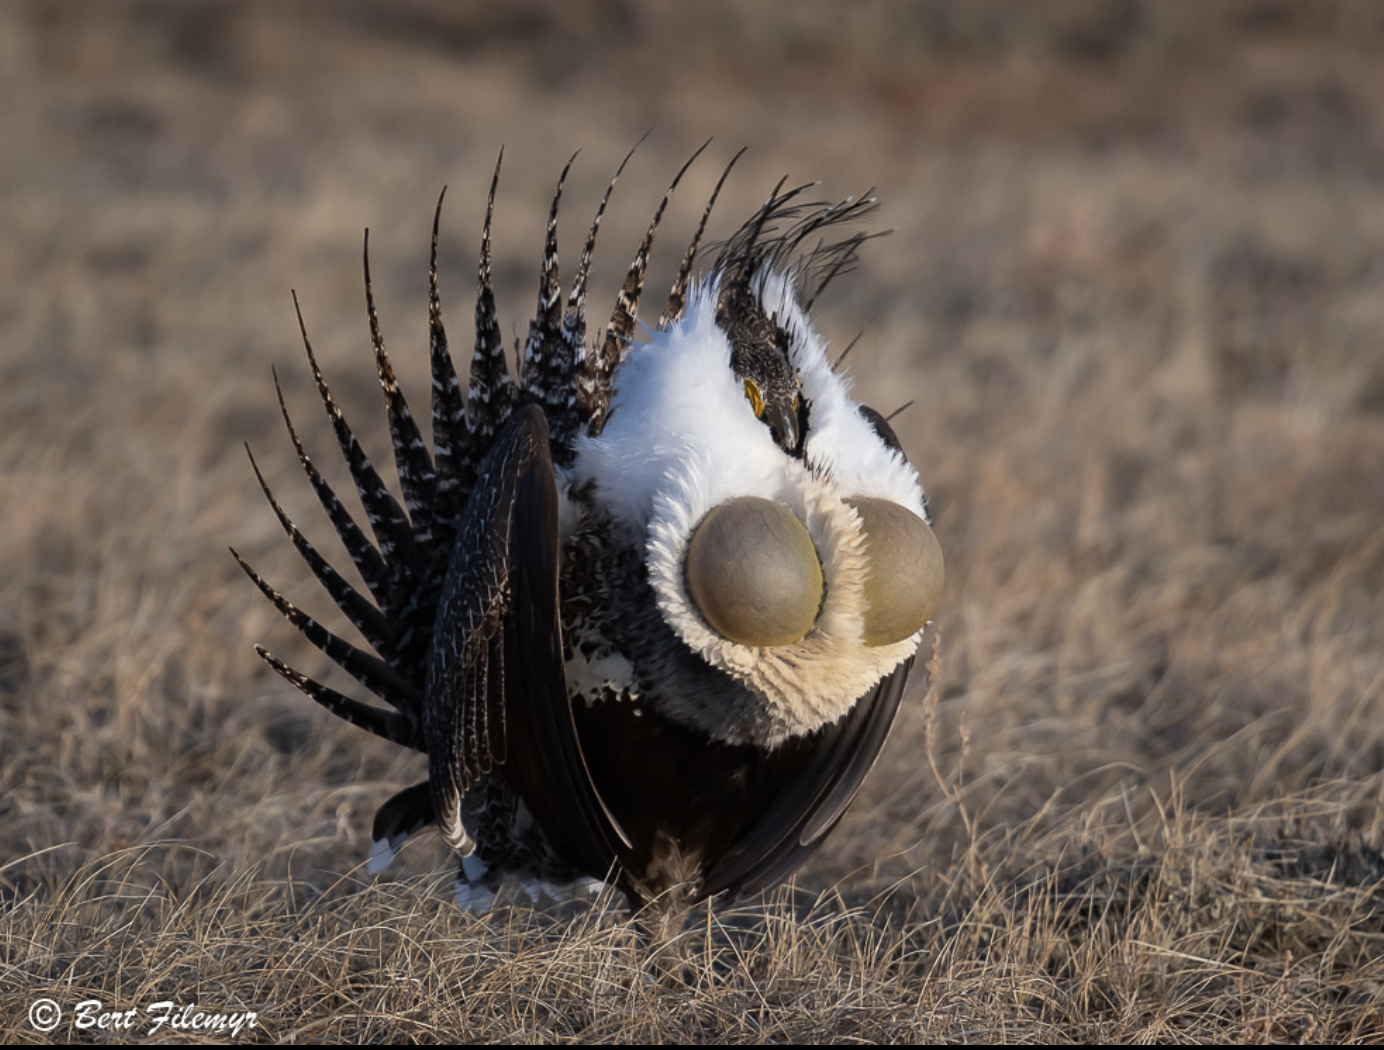
\includegraphics[width=0.5\textwidth,height=\textheight]{pic_grouse.png}

Picture: Bert Filemyr

Let's take a look at it now.

\begin{Shaded}
\begin{Highlighting}[]
\CommentTok{\# Load and examine the data}
\NormalTok{datum }\OtherTok{\textless{}{-}} \FunctionTok{read.csv}\NormalTok{(}\StringTok{"lecture\_10\_seasons.csv"}\NormalTok{)}
\FunctionTok{head}\NormalTok{(datum)}
\end{Highlighting}
\end{Shaded}

\textbf{Y-variable -- mass}

\textbf{X-variable -- season (4 groups)}

The data have the mass of animals measured in four different season:
spring, summer, fall, and winter. We have a categorical X-variable
``Season'', and also dummy-coded variables for each of the individual
seasons.

\subsubsection{The number of
comparisons}\label{the-number-of-comparisons}

Our goal is to estimate if mass of the animal is different between the
seasons. How many comparisons might we need to make?

Here's a trick to do it!

Fall Spring Summer Winter

\begin{enumerate}
\def\labelenumi{\arabic{enumi})}
\tightlist
\item
  Draw a line connecting all the neighbors.
\item
  Draw a line connecting all the two-neighbors away.
\item
  Draw a line connecting all the three-neighbors away.
\item
  Etc.
\item
  Then add up all the lines!
\end{enumerate}

In this case, we might have to do \textbf{6 pairwise comparisons}.

\subsubsection{Linear model}\label{linear-model}

Let's write out our linear model:

\textbf{\(Mass = \beta_0 + \beta_1 Spring + \beta_2 Summer + \beta_3 Winter + \epsilon \sim N(0, \sigma)\)}

\textbf{Review each of the betas}

\begin{itemize}
\tightlist
\item
  \beta\_0 -- average mass in the fall
\item
  \beta\_1 -- difference in mass between spring and fall
\item
  \beta\_2 -- difference in mass between summer and fall
\item
  \beta\_3 -- difference in mass between winter and fall
\item
  If we want to know other differences, we have to change the references
  and re-run.
\end{itemize}

What are the `true' values?

\begin{itemize}
\tightlist
\item
  \textbf{\(\beta_0\) = 4.6}
\item
  \textbf{\(\beta_1\) = \(\beta_2\) = -0.6}
\item
  \textbf{\(\beta_3\) = -0.05}
\end{itemize}

\subsubsection{Analysis in R}\label{analysis-in-r}

Let's analyze these data in R:

\begin{Shaded}
\begin{Highlighting}[]
\CommentTok{\# Plot the data}
\NormalTok{datum}\SpecialCharTok{$}\NormalTok{Season }\OtherTok{\textless{}{-}} \FunctionTok{factor}\NormalTok{(datum}\SpecialCharTok{$}\NormalTok{Season)}
\FunctionTok{plot}\NormalTok{(Mass }\SpecialCharTok{\textasciitilde{}}\NormalTok{ Season, }\AttributeTok{data =}\NormalTok{ datum)}
\end{Highlighting}
\end{Shaded}

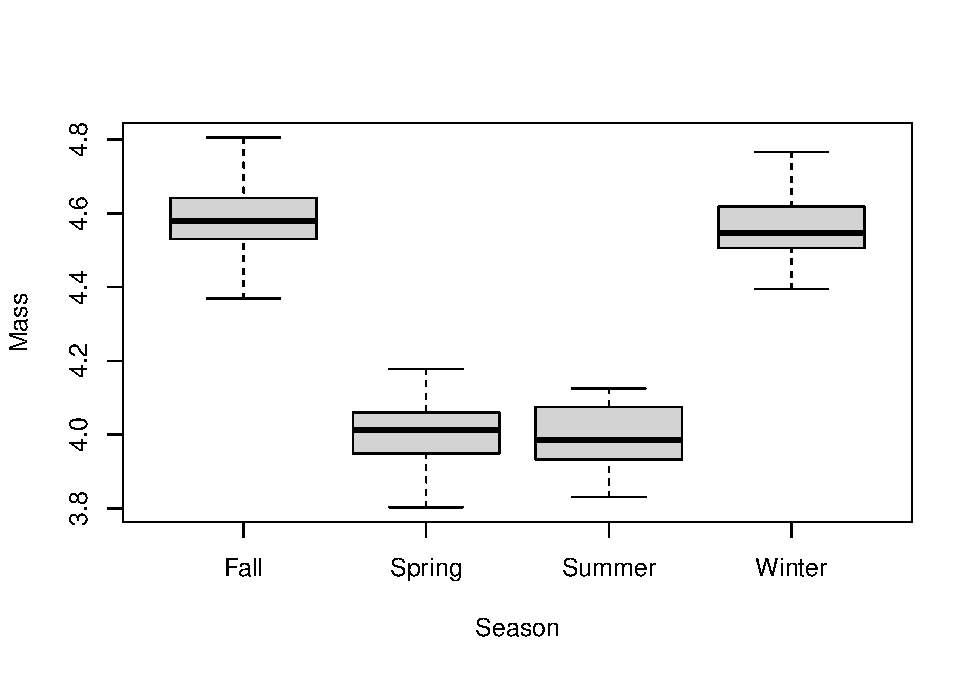
\includegraphics{lecture_10_files/figure-latex/seasons-2-1.pdf}

\begin{Shaded}
\begin{Highlighting}[]
\CommentTok{\# Fit a linear model}
\NormalTok{results }\OtherTok{\textless{}{-}} \FunctionTok{lm}\NormalTok{(Mass }\SpecialCharTok{\textasciitilde{}}\NormalTok{ Season, }\AttributeTok{data =}\NormalTok{ datum)}
\FunctionTok{summary}\NormalTok{(results)}
\end{Highlighting}
\end{Shaded}

\begin{verbatim}
## 
## Call:
## lm(formula = Mass ~ Season, data = datum)
## 
## Residuals:
##     Min      1Q  Median      3Q     Max 
## -0.2189 -0.0588 -0.0051  0.0577  0.2170 
## 
## Coefficients:
##              Estimate Std. Error t value Pr(>|t|)    
## (Intercept)    4.5880     0.0209  219.40   <2e-16 ***
## SeasonSpring  -0.5738     0.0296  -19.40   <2e-16 ***
## SeasonSummer  -0.5931     0.0296  -20.06   <2e-16 ***
## SeasonWinter  -0.0274     0.0296   -0.93     0.36    
## ---
## Signif. codes:  0 '***' 0.001 '**' 0.01 '*' 0.05 '.' 0.1 ' ' 1
## 
## Residual standard error: 0.0935 on 76 degrees of freedom
## Multiple R-squared:  0.907,  Adjusted R-squared:  0.904 
## F-statistic:  248 on 3 and 76 DF,  p-value: <2e-16
\end{verbatim}

Because we only have one variable (`Season'), the p-value in the bottom
right is the same as the p-value we would get running an ANOVA. This
gives us the significance of the season variable as a whole: it tells us
that at least two groups within this variale are different from each
other.

When we examining the significance of effects within the model, we can
see that mass in the Spring is different from Fall and that mass in the
Summer is different from Fall.

\textbf{Trick question:} Is Winter different from Fall?

Yes, it is! We simulated it to have an effect of -0.05. However, we are
not able to detect that effect with this statistical analysis. We need
to be careful to not distinguish biological from statistical
significance. We know that Winter is different from Fall, we made the
data.

\textbf{Q:} If we wanted to be sure to detect this, what would we have
to do? Increase our sample size.

Betas are all pretty close to truth.

\textbf{Q:} How would we test for the difference between Spring and
Summer?

Change the reference.

\begin{Shaded}
\begin{Highlighting}[]
\CommentTok{\# Fit a linear model}
\NormalTok{results2 }\OtherTok{\textless{}{-}} \FunctionTok{lm}\NormalTok{(Mass }\SpecialCharTok{\textasciitilde{}} \FunctionTok{relevel}\NormalTok{(Season, }\AttributeTok{ref=}\StringTok{"Summer"}\NormalTok{), }\AttributeTok{data =}\NormalTok{ datum)}
\FunctionTok{summary}\NormalTok{(results2)}
\end{Highlighting}
\end{Shaded}

\begin{verbatim}
## 
## Call:
## lm(formula = Mass ~ relevel(Season, ref = "Summer"), data = datum)
## 
## Residuals:
##     Min      1Q  Median      3Q     Max 
## -0.2189 -0.0588 -0.0051  0.0577  0.2170 
## 
## Coefficients:
##                                       Estimate Std. Error t value Pr(>|t|)    
## (Intercept)                             3.9949     0.0209  191.04   <2e-16 ***
## relevel(Season, ref = "Summer")Fall     0.5931     0.0296   20.06   <2e-16 ***
## relevel(Season, ref = "Summer")Spring   0.0193     0.0296    0.65     0.52    
## relevel(Season, ref = "Summer")Winter   0.5658     0.0296   19.13   <2e-16 ***
## ---
## Signif. codes:  0 '***' 0.001 '**' 0.01 '*' 0.05 '.' 0.1 ' ' 1
## 
## Residual standard error: 0.0935 on 76 degrees of freedom
## Multiple R-squared:  0.907,  Adjusted R-squared:  0.904 
## F-statistic:  248 on 3 and 76 DF,  p-value: <2e-16
\end{verbatim}

Now we can see other differences: summer and spring, summer and winter.

We just have to re-run this one more time to get the final comparison
that we need.

\subsubsection{Tukey's HSD}\label{tukeys-hsd}

Let's start by examining the help file for `TukeyHSD()'.

\begin{Shaded}
\begin{Highlighting}[]
\CommentTok{\# Help file}
\FunctionTok{help}\NormalTok{(TukeyHSD)}

\CommentTok{\# Tukey requires an ANOVA output}
\NormalTok{results3 }\OtherTok{\textless{}{-}} \FunctionTok{aov}\NormalTok{(Mass }\SpecialCharTok{\textasciitilde{}}\NormalTok{ Season, }\AttributeTok{data =}\NormalTok{ datum) }\CommentTok{\# or}
\NormalTok{results3 }\OtherTok{\textless{}{-}} \FunctionTok{aov}\NormalTok{(results)}
\FunctionTok{summary}\NormalTok{(results3)}
\end{Highlighting}
\end{Shaded}

\begin{verbatim}
##             Df Sum Sq Mean Sq F value Pr(>F)    
## Season       3   6.50   2.168     248 <2e-16 ***
## Residuals   76   0.66   0.009                   
## ---
## Signif. codes:  0 '***' 0.001 '**' 0.01 '*' 0.05 '.' 0.1 ' ' 1
\end{verbatim}

\begin{Shaded}
\begin{Highlighting}[]
\CommentTok{\# This analysis is so simple that it doesn\textquotesingle{}t even have a summary file. Run it directly.}
\FunctionTok{TukeyHSD}\NormalTok{(results3)}
\end{Highlighting}
\end{Shaded}

\begin{verbatim}
##   Tukey multiple comparisons of means
##     95% family-wise confidence level
## 
## Fit: aov(formula = results)
## 
## $Season
##                   diff      lwr      upr  p adj
## Spring-Fall   -0.57385 -0.65153 -0.49616 0.0000
## Summer-Fall   -0.59313 -0.67082 -0.51545 0.0000
## Winter-Fall   -0.02736 -0.10504  0.05032 0.7915
## Summer-Spring -0.01929 -0.09697  0.05839 0.9145
## Winter-Spring  0.54649  0.46880  0.62417 0.0000
## Winter-Summer  0.56577  0.48809  0.64346 0.0000
\end{verbatim}

Let's compare that to our original `lm()' results:

\begin{Shaded}
\begin{Highlighting}[]
\FunctionTok{summary}\NormalTok{(results)}
\end{Highlighting}
\end{Shaded}

\begin{verbatim}
## 
## Call:
## lm(formula = Mass ~ Season, data = datum)
## 
## Residuals:
##     Min      1Q  Median      3Q     Max 
## -0.2189 -0.0588 -0.0051  0.0577  0.2170 
## 
## Coefficients:
##              Estimate Std. Error t value Pr(>|t|)    
## (Intercept)    4.5880     0.0209  219.40   <2e-16 ***
## SeasonSpring  -0.5738     0.0296  -19.40   <2e-16 ***
## SeasonSummer  -0.5931     0.0296  -20.06   <2e-16 ***
## SeasonWinter  -0.0274     0.0296   -0.93     0.36    
## ---
## Signif. codes:  0 '***' 0.001 '**' 0.01 '*' 0.05 '.' 0.1 ' ' 1
## 
## Residual standard error: 0.0935 on 76 degrees of freedom
## Multiple R-squared:  0.907,  Adjusted R-squared:  0.904 
## F-statistic:  248 on 3 and 76 DF,  p-value: <2e-16
\end{verbatim}

\begin{itemize}
\tightlist
\item
  The difference between spring and fall is: -0.57
\item
  The difference between summer and fall is: -0.59
\item
  Point being: Tukey's HSD does not change the betas!
\end{itemize}

The `diff' is the difference between the groups. The first columns tells
us those exact differences: e.g., ``Spring - Fall''.

We can use the `lwr' and `upr' to calculate 95\% CI, as we have done
before.

Let's look at the p-values.

\begin{itemize}
\tightlist
\item
  Winter-to-Fall was 0.358, but Tukey's says it is 0.79.
\item
  Etc.
\end{itemize}

Tukey's causes \textbf{p-values get larger}.

Let's look at confidence intervals:

\begin{Shaded}
\begin{Highlighting}[]
\FunctionTok{TukeyHSD}\NormalTok{(results3)}
\end{Highlighting}
\end{Shaded}

\begin{verbatim}
##   Tukey multiple comparisons of means
##     95% family-wise confidence level
## 
## Fit: aov(formula = results)
## 
## $Season
##                   diff      lwr      upr  p adj
## Spring-Fall   -0.57385 -0.65153 -0.49616 0.0000
## Summer-Fall   -0.59313 -0.67082 -0.51545 0.0000
## Winter-Fall   -0.02736 -0.10504  0.05032 0.7915
## Summer-Spring -0.01929 -0.09697  0.05839 0.9145
## Winter-Spring  0.54649  0.46880  0.62417 0.0000
## Winter-Summer  0.56577  0.48809  0.64346 0.0000
\end{verbatim}

\begin{Shaded}
\begin{Highlighting}[]
\FunctionTok{confint}\NormalTok{(results)}
\end{Highlighting}
\end{Shaded}

\begin{verbatim}
##                 2.5 %   97.5 %
## (Intercept)   4.54636  4.62966
## SeasonSpring -0.63275 -0.51495
## SeasonSummer -0.65203 -0.53423
## SeasonWinter -0.08626  0.03154
\end{verbatim}

Compare Spring-Fall from both outputs.

\begin{Shaded}
\begin{Highlighting}[]
\CommentTok{\# Spring to Fall}
\NormalTok{(}\SpecialCharTok{{-}}\FloatTok{0.63274618} \SpecialCharTok{{-}} \SpecialCharTok{{-}}\FloatTok{0.5149456}\NormalTok{)}\SpecialCharTok{/}\DecValTok{2} \CommentTok{\# LM}
\end{Highlighting}
\end{Shaded}

\begin{verbatim}
## [1] -0.0589
\end{verbatim}

\begin{Shaded}
\begin{Highlighting}[]
\NormalTok{(}\SpecialCharTok{{-}}\FloatTok{0.65152888} \SpecialCharTok{{-}} \SpecialCharTok{{-}}\FloatTok{0.49616295}\NormalTok{)}\SpecialCharTok{/}\DecValTok{2} \CommentTok{\#Tukey}
\end{Highlighting}
\end{Shaded}

\begin{verbatim}
## [1] -0.07768
\end{verbatim}

Tukey causes \textbf{confidence intervals to become wider}.

\textbf{Takehome:} Both the p-values and confidence intervals have
become artificially inflated.

\subsubsection{Cautionary tale}\label{cautionary-tale}

Sometimes people take a categorical variable and they turn it into a
continuous variable. This can be dangerous! Take a look:

\begin{Shaded}
\begin{Highlighting}[]
\CommentTok{\# Look at the second to last column}
\FunctionTok{head}\NormalTok{(datum)}
\end{Highlighting}
\end{Shaded}

They then run a model with that as the predictor variable.

\begin{Shaded}
\begin{Highlighting}[]
\CommentTok{\# Run a \textquotesingle{}lm()\textquotesingle{} with that}
\NormalTok{results4 }\OtherTok{\textless{}{-}} \FunctionTok{lm}\NormalTok{(Mass }\SpecialCharTok{\textasciitilde{}}\NormalTok{ SeasonN, }\AttributeTok{data =}\NormalTok{ datum)}
\FunctionTok{summary}\NormalTok{(results4)}
\end{Highlighting}
\end{Shaded}

\begin{verbatim}
## 
## Call:
## lm(formula = Mass ~ SeasonN, data = datum)
## 
## Residuals:
##    Min     1Q Median     3Q    Max 
## -0.370 -0.109 -0.001  0.122  0.361 
## 
## Coefficients:
##             Estimate Std. Error t value Pr(>|t|)    
## (Intercept)   4.8709     0.0411   118.4   <2e-16 ***
## SeasonN      -0.2326     0.0150   -15.5   <2e-16 ***
## ---
## Signif. codes:  0 '***' 0.001 '**' 0.01 '*' 0.05 '.' 0.1 ' ' 1
## 
## Residual standard error: 0.15 on 78 degrees of freedom
## Multiple R-squared:  0.755,  Adjusted R-squared:  0.751 
## F-statistic:  240 on 1 and 78 DF,  p-value: <2e-16
\end{verbatim}

Season is significant! They write that in their paper and send it in for
publication and they are done.

But they made a lot of errors here.

\begin{itemize}
\tightlist
\item
  First, they focused too much on p-values.
\item
  If they would have been thinking about effects between groups (betas),
  they might have realized the issue.
\end{itemize}

\textbf{Q:} What did R do?

It ran a regression with two continuous variables, X as a continuous
variable. This assumes there is a linear relationship between 1, 2, 3, 4
and mass. That might be valid\ldots{} but it isn't!

\begin{Shaded}
\begin{Highlighting}[]
\CommentTok{\# Scatterplot}
\FunctionTok{plot}\NormalTok{(Mass }\SpecialCharTok{\textasciitilde{}}\NormalTok{ SeasonN, }\AttributeTok{data =}\NormalTok{ datum)}
\end{Highlighting}
\end{Shaded}

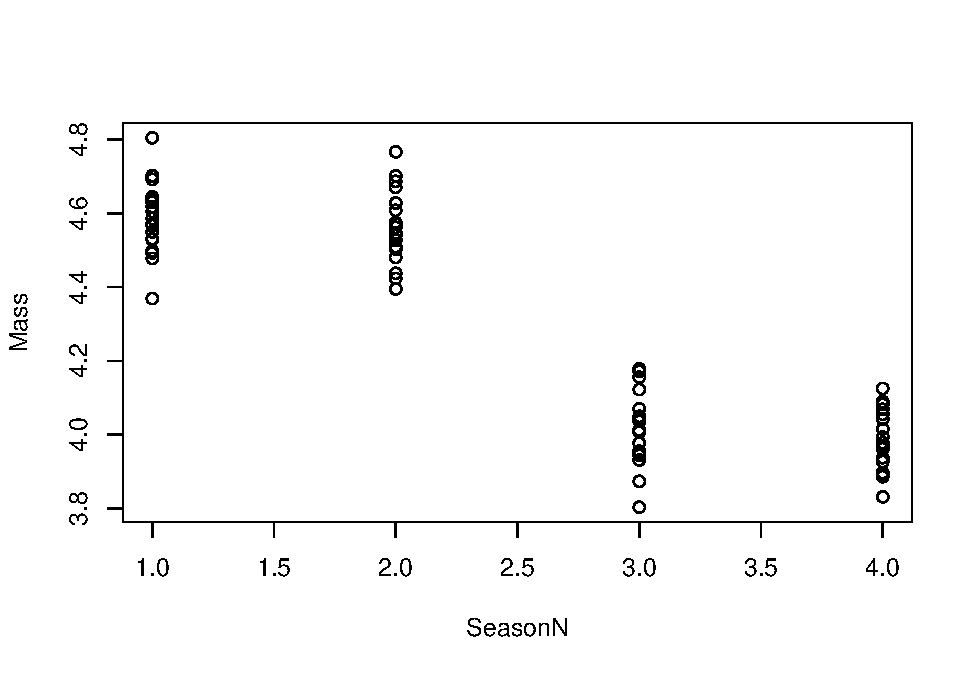
\includegraphics{lecture_10_files/figure-latex/seasons-10-1.pdf}

\textbf{Q:} How do we know it ran it as a regression?

It only gave us a single beta, and it only used 1 degree of freedom
(should have been 3).

A post-hoc test\ldots{} won't work:

\begin{Shaded}
\begin{Highlighting}[]
\CommentTok{\# Scatterplot}
\CommentTok{\#TukeyHSD(aov(results4)) \# doesn\textquotesingle{}t work!}
\CommentTok{\# Error in \textasciigrave{}TukeyHSD.aov()\textasciigrave{}:}
\CommentTok{\# ! no factors in the fitted model}
\end{Highlighting}
\end{Shaded}

R is trying to tell us that `Season' is not a number -- it is a
`factor'.

\textbf{factor -- a categorical X-variable}

\textbf{covariate -- a continuous X-variable in a statistical model}

Two terms we should be aware of.

\subsection{Summary}\label{summary}

We need to know that there are these things called `post-hoc tests'.

They try to maintain the `experiment-wide error rate' (0.05 Type 1 error
rate), and are still used a lot, particularly in classic agricultural or
fisheries journals if you have done a manipulative experiment.

As you build more complicated models that have more complicated models
(with both categorical and continuous variables), post-hoc tests won't
work.

Bonferonni corrections (basic math) can be used if absolutely necessary.

\subsection{Truth}\label{truth}

Here is code to simulate the data we analyzed in this lecture.

\begin{Shaded}
\begin{Highlighting}[]
\DocumentationTok{\#\#\# Lecture 10: code to simulate data for post{-}hoc tests }

\CommentTok{\# Set the seed for reproducibility}
\FunctionTok{set.seed}\NormalTok{(}\DecValTok{123}\NormalTok{)}

\CommentTok{\# Simulate X{-}variable}
\NormalTok{n }\OtherTok{\textless{}{-}} \DecValTok{80}
\NormalTok{x }\OtherTok{\textless{}{-}} \FunctionTok{factor}\NormalTok{(}\FunctionTok{c}\NormalTok{(}\FunctionTok{rep}\NormalTok{(}\StringTok{"Spring"}\NormalTok{, n}\SpecialCharTok{/}\DecValTok{4}\NormalTok{), }\FunctionTok{rep}\NormalTok{(}\StringTok{"Summer"}\NormalTok{, n}\SpecialCharTok{/}\DecValTok{4}\NormalTok{), }\FunctionTok{rep}\NormalTok{(}\StringTok{"Winter"}\NormalTok{, n}\SpecialCharTok{/}\DecValTok{4}\NormalTok{), }\FunctionTok{rep}\NormalTok{(}\StringTok{"Fall"}\NormalTok{, n}\SpecialCharTok{/}\DecValTok{4}\NormalTok{)))}

\CommentTok{\# Season as a numeric}
\NormalTok{SeasonN }\OtherTok{\textless{}{-}} \FunctionTok{as.numeric}\NormalTok{(}\FunctionTok{factor}\NormalTok{(x, }\AttributeTok{levels =} \FunctionTok{c}\NormalTok{(}\StringTok{"Fall"}\NormalTok{, }\StringTok{"Winter"}\NormalTok{, }\StringTok{"Spring"}\NormalTok{, }\StringTok{"Summer"}\NormalTok{)))}

\CommentTok{\# Simulate error}
\NormalTok{error }\OtherTok{\textless{}{-}} \FunctionTok{rnorm}\NormalTok{(n, }\AttributeTok{mean =} \DecValTok{0}\NormalTok{, }\AttributeTok{sd =} \FloatTok{0.1}\NormalTok{)}

\CommentTok{\# Create dummy{-}coded variables}
\NormalTok{dummy }\OtherTok{\textless{}{-}} \FunctionTok{model.matrix}\NormalTok{(}\SpecialCharTok{\textasciitilde{}}\NormalTok{ x }\SpecialCharTok{{-}} \DecValTok{1}\NormalTok{)}
\FunctionTok{colnames}\NormalTok{(dummy) }\OtherTok{\textless{}{-}} \FunctionTok{c}\NormalTok{(}\StringTok{"Fall"}\NormalTok{, }\StringTok{"Spring"}\NormalTok{, }\StringTok{"Summer"}\NormalTok{, }\StringTok{"Winter"}\NormalTok{)}

\CommentTok{\# Create the dataframe}
\NormalTok{datum }\OtherTok{\textless{}{-}} \FunctionTok{data.frame}\NormalTok{(}\AttributeTok{Season =}\NormalTok{ x, }\AttributeTok{error =}\NormalTok{ error, dummy, SeasonN)}

\CommentTok{\# Calculate Y{-}variable}
\NormalTok{y }\OtherTok{\textless{}{-}} \FloatTok{4.6} \SpecialCharTok{{-}}\NormalTok{ (}\FloatTok{0.6} \SpecialCharTok{*}\NormalTok{ datum}\SpecialCharTok{$}\NormalTok{Spring) }\SpecialCharTok{{-}}\NormalTok{ (}\FloatTok{0.6} \SpecialCharTok{*}\NormalTok{ datum}\SpecialCharTok{$}\NormalTok{Summer) }\SpecialCharTok{{-}}\NormalTok{ (}\FloatTok{0.05} \SpecialCharTok{*}\NormalTok{ datum}\SpecialCharTok{$}\NormalTok{Winter) }\SpecialCharTok{+}\NormalTok{ error}

\CommentTok{\# Create dataframe}
\NormalTok{datum }\OtherTok{\textless{}{-}} \FunctionTok{cbind}\NormalTok{(datum, }\AttributeTok{Mass =}\NormalTok{ y)}

\CommentTok{\# Save the CSV file}
\FunctionTok{write.csv}\NormalTok{(datum, }\StringTok{"lecture\_10\_seasons.csv"}\NormalTok{, }\AttributeTok{row.names =} \ConstantTok{FALSE}\NormalTok{)}
\end{Highlighting}
\end{Shaded}

\href{lecture_11.html}{--go to next lecture--}

\end{document}
